\chapter{Static Analysis (WORK IN PROGRESS)}
\label{static-analysis}

This chapter describes static code analysis, the difference to other analysis types, the technical details and the theory behind it.

\section{Static Analysis vs.~Dynamic Analysis}

Generally, there are two basic approaches to program analysis, differentiated by the time of the analysis: \emph{static analysis} and \emph{dynamic analysis}.

\subsection{Static Analysis}
\index{static analysis}\index{SA\see{static analysis}}\index{static code analysis|see{static analysis}}

\emph{Static analysis (SA)} or \emph{Static code analysis} is defined as analyzing the way code of a program (the source code, byte code or machine code) will execute instead of---or before---actually running it. The analysis is performed on an abstract level, i.e., it does not use concrete data for checking.~\cite{static-code-analysis}

The aim of static analysis is to find bugs, structural problems, code smells or to help in understanding the system that is analyzed very early in the development cycle.~\cite{data-flow-analysis, chess-west} Optimally, the developer will be able to see the problems directly during development, e.g., as markers in their development environment, or as feedback from a tool that is run in parallel.

Static analysis allows all possible program paths to be checked, independent of whether the program paths actually are executed during the particular set of data used during execution. In addition, the results of static code analysis are repeatable.~\cite{coverity-report}

\subsection{Dynamic Analysis}
\index{dynamic analysis}

\emph{Dynamic analysis} is code analysis that happens when the code actually is executed. This usually comes with a performance penalty, but is also increases precision because the analysis works on the actual data instead of a general model of the data.~\cite{chess-west} However, it also considerably reduces the callback as the dynamic analysis always works on a concrete set of data, and the analysis will not find problems that only occur with different data.~\cite{static-code-analysis}

Examples of automated dynamic analysis would be penetration tests (for the outside view) or unit tests.



\section{Approaches to Static Analysis}
Generally, there are several different approaches when doing static code analysis~\cite{comparison-of-bug-finding-tools}: string pattern matching, syntactic bug pattern detection, data-flow analysis, theorem proving and model checking.


\subsection{String Pattern Matching}
\index{string pattern matching}

\emph{String pattern matching} is the most simple form of static code analysis. With this approach, the scanner approaches the program basically just as list of lines, which consist of characters. This kind of scanner does not operate on tokens or any other abstracted structure of the program.

The scanner checks for security vulnerabilities by scanning for certain commands or command sequences and heavily relies on the human eye for filtering out false positives. This greatly reduces its practical use as programmers tend to ignore warnings if they contains lots of false positives.~\cite{understanding-value}

Still, it is possible to use this approach for finding some vulnerabilities, for example using \emph{Google Code Search}\index{Google Code Search}.~\cite{google-code-search}

The main drawback of this approach is that there are lots of false positives (e.g., with the tool SWAAT~\cite{swaat}) as the tools do not use any data-flow analysis and thus cannot differentiate between a potentially unsafe command being executed with data that is really unsafe and those cases where the data at is ensured to be safe that point.

The most basic way of applying this code analysis is by just using the text search function of a text editor (with or without regular expressions)\index{regular expressions}) or text-search command line tools like \emph{grep}.


\subsection{Syntactic Bug Pattern Detection (``Style Checking'')}
\index{style checking}\index{syntactic bug pattern detection}

Syntactic bug pattern detection means the scanner works a model of the code and its structure, for example a stream of tokens or an abstract syntax tree. However, this kind of scanner does not apply any interprocedural control-flow or data-flow analysis. This type of scanner often is used for enforcing coding style guidelines, e.g., in continuous integration (CI)\index{continuous integration} environments like Jenkins. Hence, these scanners also are called ``style checkers''.

Compared to string pattern matching for finding bugs, this approach greatly reduces the number of false positives and makes the scanner a lot more useful.~\cite{comparison-of-bug-finding-tools}. Tools like \emph{PHPCodeSniffer}\index{PHPCodeSniffer}, \emph{PMD}\index{PMD} or \emph{FindBugs}\index{FindBugs} fall into this category.


\subsection{Data-Flow Analysis}
\index{data-flow analysis}\index{control-flow analysis}

Scanners that rely on data-flow analysis first create information about the control flow, i.e., about the possible paths through the program. On top of this information, they compute information about the what data is used or modified at which program point.~\cite{data-flow-analysis} This information usually is an approximation of the real data that is used during program execution.

Data flow analysis consists of \emph{intraproceducal data-flow analysis}\index{intraproceducal data-flow analysis} (i.e., the analysis of the data flow within a function and in the global scope) and \emph{interproceducal data-flow analysis}\index{interproceducal data-flow analysis} (i.e., the analysis of the data flow between functions).

Data-flow analysis is the most precise way of scanning statically for security vulnerabilities without having to annotate the source code in any way.

\emph{Pixy}~\cite{pixy} is an example of a security scanner using data-flow analysis.


\subsection{Theorem Proving}
\index{theorem proving}

\emph{Theorem proving} relies on the programmer adding preconditions, postconditions and loop invariants to the source code as code annotations. The scanner then can analyze the program and check whether all conditions are met.~\cite{comparison-of-bug-finding-tools}

\emph{ESC/Java}\index{ESC/Java} is an example for this class of tools.


\subsection{Model Checking}
\index{model checking}

Model checking relies on creating suitable models of the program---either by hand or automatically, using code annotations that state what should be checked.~\cite{data-flow-analysis} One drawback of this class of scanners is that programs that include library calls are practically impossible to check, which greatly reduces the applicability of this approach for real-world programs.~\cite{comparison-of-bug-finding-tools}

\emph{Bandera}\index{Bandera} is a scanner that makes use of model checking.


\section{Static Analysis for Finding Vulnerabilities}

Tools for static code analysis can find real bugs in production software \cite{findbugs, evaluating}, including security problems like unintentionally ignored expressions, use-after-free or buffer overflows. Coverty~\cite{coverity-report}\index{Coverity} regularly use their scanner to scan some open source projects for free, provide the bug reports to the projects, and publish regular reports on their efforts and the results, including numbers on the different vulnerability types found by their tool.

\cite{chess-west} explains in detail how static analysis of code works and how it can be used to find bugs and vulnerabilities.



\section{Tainted Object Propagation}
\label{tainting}\index{tainted object propagation}
\cite{finding-security-vulnerabilities} describes an approach to finding a class of vulnerabilities called \emph{tainted object propagation}. \cite{pixy-short, pixy-long, pixy-dissertation} apply this to PHP.

Tainted object propagation builds on data-flow analysis and traces where untrusted data comes into the system and where it is used. Pixy implements this approach.

The concepts of this approach are as following:
\paragraph{Sources} are the places where potentially malicious data comes in. In the example (figure \ref{fig:taint} on page \pageref{fig:taint}), the \texttt{\$\_GET} variable ``name'' is a source.\index{source}
\paragraph{Tainted} means that data is considered to be potentially dangerous.\index{tainting}
\paragraph{Sinks} are the places where the data is used and where tainted data could cause harm. In the example (figure \ref{fig:taint} on page \pageref{fig:taint}), the \texttt{echo} call is a sink.\index{sink}

\begin{figure}[!h]
  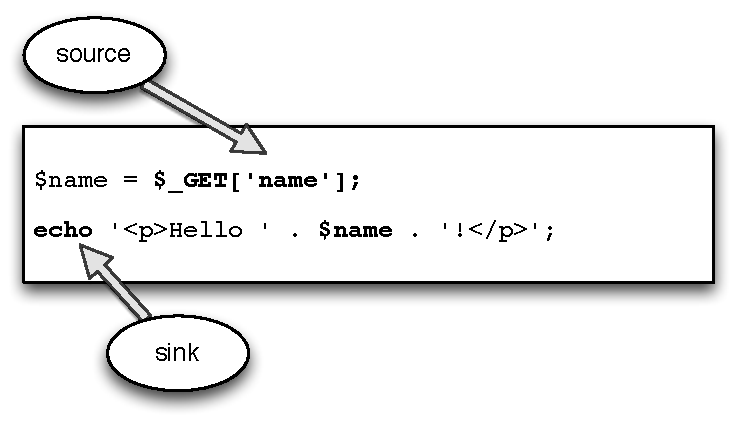
\includegraphics[scale=0.8]{images/taint}
  \caption{Tainted data can be traced on its way from the source to the sink.}
  \label{fig:taint}
\end{figure}

\paragraph{Sanitizing} tainted data from a source changes it so that it will not cause any harm when put into a sink. In the second example (figure \ref{fig:taint-and-clean} on page \pageref{fig:taint-and-clean}), the \texttt{htmlspecialchars} call sanitized the tainted data.\index{sanitizing}\index{sanitation|see{sanitizing}}

\begin{figure}[!h]
 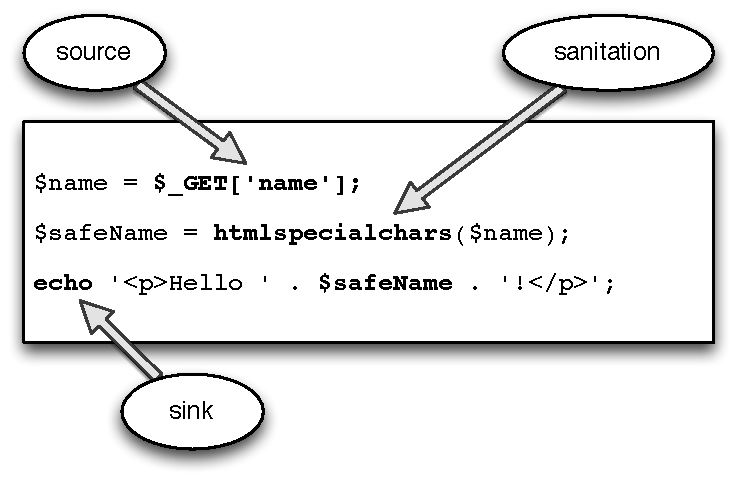
\includegraphics[scale=0.8]{images/taint-and-clean}
 \caption{Tainted data gets sanitized on its way from the source to the sink.}
 \label{fig:taint-and-clean}
\end{figure}

